%%%%%%%%%%%%%%%%%%%%%%%%%%%%%%%%%%%%%%%%%
% Beamer Presentation
% LaTeX Template
% Version 1.0 (10/11/12)
%
% This template has been downloaded from:
% http://www.LaTeXTemplates.com
%
% License:
% CC BY-NC-SA 3.0 (http://creativecommons.org/licenses/by-nc-sa/3.0/)
%
%%%%%%%%%%%%%%%%%%%%%%%%%%%%%%%%%%%%%%%%%

%----------------------------------------------------------------------------------------
%    PACKAGES AND THEMES
%----------------------------------------------------------------------------------------

\documentclass{beamer}

\mode<presentation> {
	
	% The Beamer class comes with a number of default slide themes
	% which change the colors and layouts of slides. Below this is a list
	% of all the themes, uncomment each in turn to see what they look like.
	
	%\usetheme{default}
	%\usetheme{AnnArbor}
	%\usetheme{Antibes}
	%\usetheme{Bergen}
	%\usetheme{Berkeley}
	%\usetheme{Berlin}
	\usetheme{Boadilla}
	%\usetheme{CambridgeUS}
	%\usetheme{Copenhagen}
	%\usetheme{Darmstadt}
	%\usetheme{Dresden}
	%\usetheme{Frankfurt}
	%\usetheme{Goettingen}
	%\usetheme{Hannover}
	%\usetheme{Ilmenau}
	%\usetheme{JuanLesPins}
	%\usetheme{Luebeck}
	%\usetheme{Madrid}
	%\usetheme{Malmoe}
	%\usetheme{Marburg}
	%\usetheme{Montpellier}
	%\usetheme{PaloAlto}
	%\usetheme{Pittsburgh}
	%\usetheme{Rochester}
	%\usetheme{Singapore}
	%\usetheme{Szeged}
	%\usetheme{Warsaw}
	
	% As well as themes, the Beamer class has a number of color themes
	% for any slide theme. Uncomment each of these in turn to see how it
	% changes the colors of your current slide theme.
	
	%\usecolortheme{albatross}
	%\usecolortheme{beaver}
	%\usecolortheme{beetle}
	%\usecolortheme{crane}
	%\usecolortheme{dolphin}
	%\usecolortheme{dove}
	%\usecolortheme{fly}
	%\usecolortheme{lily}
	%\usecolortheme{orchid}
	%\usecolortheme{rose}
	%\usecolortheme{seagull}
	%\usecolortheme{seahorse}
	%\usecolortheme{whale}
	%\usecolortheme{wolverine}
	
	%\setbeamertemplate{footline} % To remove the footer line in all slides uncomment this line
	\setbeamertemplate{footline}[page number] % To replace the footer line in all slides with a simple slide count uncomment this line
	
	\setbeamertemplate{navigation symbols}{} % To remove the navigation symbols from the bottom of all slides uncomment this line
}

\usepackage{subcaption, picture, graphicx} % Allows including images
\graphicspath{{pictures/}}
\usepackage{booktabs} % Allows the use of \toprule, \midrule and \bottomrule in tables
\usepackage{multirow}
\usepackage{natbib}


\usepackage{xcolor}
\usepackage[outputdir=../]{minted}
\usepackage{pdflscape}
\usepackage{tikz} 
\usetikzlibrary{matrix}
\newcommand{\red}{\color{red}}
\newcommand{\blue}{\color{blue}}

\usepackage{bm}
\usepackage{amsmath, amsthm, amssymb, amsthm, amsfonts}
\newcommand{\bbeta}{\bm{\beta}}
\newcommand{\btheta}{\bm{\theta}}
\newcommand{\htheta}{\hat{\bm{\theta}}}
\newcommand{\x}{\bm{x}}
\newcommand{\X}{\bm{X}}
\newcommand{\y}{\bm{y}}
\newcommand{\z}{\bm{z}}
\newcommand{\tp}{^{\mathrm{T}}}
\newcommand{\bdelta}{\bm{\delta}}
\newcommand{\bt}{\bm{t}}
\newcommand{\pr}{\mathbb{P}}

\newcommand{\rhl}[1]{{\red \textbf{#1}}}
\newcommand{\bhl}[1]{{\blue \textbf{#1}}}

%----------------------------------------------------------------------------------------
%    TITLE PAGE
%----------------------------------------------------------------------------------------

\title[Survival Analysis]{Investigation on imbalanced Cox regression based on simulations} % The short title appears at the bottom of every slide, the full title is only on the title page

\author{Jing Wang} % Your name
\institute[UConn] % Your institution as it will appear on the bottom of every slide, may be shorthand to save space
{
	University of Connecticut \\ % Your institution for the title page
	\medskip
}
\date{\today} % Date, can be changed to a custom date

\begin{document}
	
	\begin{frame}
		\titlepage % Print the title page as the first slide
	\end{frame}
	
	\begin{frame}
		\frametitle{Overview} % Table of contents slide, comment this block out to remove it
		\tableofcontents % Throughout your presentation, if you choose to use \section{} and \subsection{} commands, these will automatically be printed on this slide as an overview of your presentation
	\end{frame}
	
	%----------------------------------------------------------------------------------------
	%    PRESENTATION SLIDES
	%----------------------------------------------------------------------------------------
	
	%------------------------------------------------
	\section{Background and paper review} % Sections can be created in order to organize your presentation into discrete blocks, all sections and subsections are automatically printed in the table of contents as an overview of the talk
	%------------------------------------------------
	
	%\subsection{Background} % A subsection can be created just before a set of slides with a common theme to further break down your presentation into chunks
	
	\begin{frame}
		\frametitle{Background}
		\begin{itemize}
		    \item Imbalanceness is an issue for binary response
            \item Recent years many techniques have been developed to rebalance the data from both statistics and machine learning perspective.
		\end{itemize}
        \begin{itemize}
            \item Survival analysis can also suffer imbalance issue
            \item Research on imbalance survival analysis is rarely touched by researchers.
        \end{itemize}
	\end{frame}

 \subsection{Existing researches on highly imbalanced logistic regression}
    \begin{frame}
        \frametitle{Paper review}
        \framesubtitle{Logistic regression}
        \begin{itemize}
            \item Logistic regression is a wildly used statistical model for \rhl{binary data}
            \item For a $y\in\{0,1\}$ and $\x$, logistic regressions assume that
            \begin{equation*}
                \pr(y=1|\x)=\frac{e^{\alpha+\x\tp\bbeta}}{1+e^{\alpha+\x\tp\bbeta}}
            \end{equation*}
            \item For this model
            \begin{itemize}
                \item Response $y$: \bhl{Yes} or \bhl{No}, \bhl{Have a disease} or \bhl{Not have a disease}
                \item Covariate $\x$: Age, Height, Weight, etc.
                \item \rhl{$\alpha$: Intercept}, $\bbeta$: coefficients of $\x$.
            \end{itemize}
        \end{itemize}
    \end{frame}
    
    \begin{frame}
        \frametitle{Paper review}
        \framesubtitle{Highly imbalanced logistic regression}
        \begin{itemize}
            \item What if $\pr(y=1)$ is very small (For example 0.5\%)?
            \begin{itemize}
                \item rare diseases, war, disaster
                \item Resultant data is highly imbalanced: rare 1 and large amount of 0
            \end{itemize}
        \end{itemize}
        \begin{itemize}
            \item \cite{wang2020logistic} proposes the following adjusted logistic regression to model highly imbalanced binary data:
            \begin{equation*}
                \pr(y=1|\x)=\frac{e^{\alpha+\x\tp\bbeta}}{1+e^{\alpha+\x\tp\bbeta}}
            \end{equation*}
            \item Assume that \rhl{$\bbeta$ is fixed and $\alpha\to-\infty$} as $N\to\infty$, then
            \begin{equation*}
                \pr(y=1)\to 0,
            \end{equation*}
            and
            \begin{equation*}
                \frac{N_1}{N}=\frac{N_1}{N_0+N_1}=\pr(y=1)\{1+o_p(1)\}\to0.
            \end{equation*}
        \end{itemize}    
    \end{frame}

    \begin{frame}
        \frametitle{Paper review}
        \framesubtitle{Estimation of highly imbalanced logistic regression}
        \begin{itemize}
            \item Denoting $\z=(1,\x\tp)\tp$ and $\btheta=(\alpha,\bbeta\tp)\tp$, the MLE estimator:
        \begin{equation*}
            \htheta=\max_{\btheta}\ell(\btheta)=\max_{\btheta}\sum_{i=1}^{N}\{y_i\z_i\tp\btheta-\log(1+e^{\z_i\tp\btheta})\}
        \end{equation*}
        is \bhl{asymptotic normal}:
        \begin{equation*}
            \htheta-\btheta_0\approx N\left(\bm{0}, \frac{\bm{V}_f}{{\red N_1}}\right).
        \end{equation*}
        \end{itemize}
        \begin{itemize}
            \item For regular logistic regression, we usually have
            \begin{equation*}
                \htheta-\btheta_0\approx N\left(\bm{0}, \frac{\bm{V}_f}{{\red N}}\right)
            \end{equation*}
            \item Information in data is essentially determined by $N_1$ instead of $N$.
        \end{itemize}
    \end{frame}

    \begin{frame}
        \frametitle{Paper review}
        \framesubtitle{Methods to balance the data}
        \begin{itemize}
            \item Imbalanceness may cause many issues in data analysis
            \item If imbalance rate is low, to get enough $N_1$, needs large amount of $N$
            \item In practice, imbalanceness may cause computational instability.
            \item In machine learning, \rhl{under-sample} and \rhl{over-sampling} is used.
        \end{itemize}
    \end{frame}

    \begin{frame}
        \frametitle{Paper review}
        \framesubtitle{Methods to balance the data}
        \begin{exampleblock}{Under-sampling}
        \begin{itemize}
            \item If $y_i=1$, include $(y_i, \x_i)$ into the sample
            \item If $y_i=0$, include $(y_i, \x_i)$ with \bhl{probability $\rho$}
        \end{itemize}
    \end{exampleblock}
    \begin{exampleblock}{Over-sampling}
        \begin{itemize}
            \item If $y_i=1$, include $(y_i, \x_i)$ into the sample $1+v$ times, where \bhl{$v\sim Poisson(\lambda)$}
            \item If $\delta_i=0$, include $(y_i, \x_i)$ only once
        \end{itemize}
    \end{exampleblock}
    \end{frame}

    \begin{frame}
        \frametitle{Paper review}
        \framesubtitle{Methods to balance the data}
        \begin{itemize}
            \item \cite{wang2020logistic} also propose two estimators based on resultant balanced data set: \rhl{weighted} and \rhl{unweighted} estimator
        \end{itemize}
        \begin{exampleblock}{Weighted method}
        \begin{itemize}
            \item Taking samples with under- (or over-) sampling with $\rho$ (or $\lambda$)
            \item If using under-sampling, weighting 0's with $\frac{1}{\rho}$, 
            \item If using over-sampling, weighting 1's with $1/(1+\lambda)$
            \item Apply weighted logistic regression on sample
        \end{itemize}
    \end{exampleblock}
    \begin{exampleblock}{Unweighted method}
        \begin{itemize}
            \item Taking samples with under- (or over-) sampling with $\rho$ (or $\lambda$)
            \item \rhl{Directly apply logistic regression on the sample and obtain $\htheta_u$}
            \item \rhl{Adjust $\hat{\alpha}=\hat{\alpha}_u+\log(\rho)$ or $\hat{\alpha}=\hat{\alpha}_u+\log(1+\lambda)$}.
        \end{itemize}
    \end{exampleblock}
    \end{frame}

    \begin{frame}
        \frametitle{Paper review}
        \framesubtitle{Methods to balance the data}
        \cite{wang2020logistic} proved the following results
        \begin{itemize}
            \item For all the 4 methods, \rhl{the asymptotic variances are of order $\frac{1}{N_1}$}.
            \item Both under- and over-sampling will cause information loss
            \item For under-sampling, when $e^\alpha/\rho\to 0$, \rhl{no information loss}
            \item For over-sampling, when $\lambda=0$ or $\infty$, \rhl{no information loss}
            \item For under-sampling. unweighted estimator with bias correction is more efficient
            \item For over-sampling. weighted estimator is more efficient
        \end{itemize}
    \end{frame}

    \subsection{Survival data}

    \begin{frame}
        \frametitle{Paper review}
        \framesubtitle{Survival data and Cox regression}
        \begin{itemize}
            \item In statistics, survival analysis studies time to a certain event
            \begin{itemize}
                \item Time to death (Survival time), marriage,...
                \item Time to develop a certain diseases
                \item Time to malfunctions of a machine
            \end{itemize}
            \item For survival analysis, due to practical issues, for example, limited resources, data usually suffer censorings
            \begin{itemize}
                \item A study follows a large amount of patients for 5 years for a certain disease. However, some patients never develop that diseases in this 5 years. Then, for those patients, we only know their $t_i>5$.
            \end{itemize}
        \end{itemize}
    \end{frame}

    \begin{frame}
        \frametitle{Paper review}
        \framesubtitle{Survival data and Cox regression}
        \begin{itemize}
            \item A survival data set usually contains three parts $(t_i,\delta_i,\x_i)$
            \begin{itemize}
                \item $t_i$: observed survival time
                \item $\delta_i$: indicator of event. If $\delta=1$, event is observed, if $\delta=0$, censoring is observed.
                \item $\x_i$: covariates related to $t_i$, for example, age, height, weight,...
            \end{itemize}
        \end{itemize}
        \begin{itemize}
            \item A popular model for survival data is the Cox model:
            \begin{equation*}
                h(t|\x)=h_0(t)e^{\x\tp\bbeta}.
            \end{equation*}
            \begin{itemize}
                \item $h(t|\x)$ called hazard function, which is the risk of event at time $t$.
                \item $h_0(t)$ is the baseline hazard function
                \item Covariates $\x$ affect survival time through affecting hazard function.
            \end{itemize}
        \end{itemize}
    \end{frame}

    \begin{frame}
        \frametitle{Paper review}
        \framesubtitle{Survival data and Cox regression}
        \begin{itemize}
            \item In Cox model, we do not assume a specific form of $h_0(t)$ and thus, there is no intercept term $\alpha$ in Cox model because 
            \begin{equation*}
                h(t|\x)=h_0(t)e^{\alpha+\x\tp\bbeta}=\tilde{h}_0(t)e^{\x\tp\bbeta},
            \end{equation*}
            where $\tilde{h}_0(t)=h_0(t)e^\alpha$ and thus $\alpha$ is not estimable. 
            \item From the above reason, we usually focus more on estimating coefficients $\bbeta$.
            \item Note that the \bhl{lower $h_0(t)$}, the \bhl{lower risk of event} and thus the \bhl{lower rate of observed events}. 
        \end{itemize}
    \end{frame}

    \begin{frame}
        \frametitle{Background}
        \framesubtitle{Some question about survival analysis}
        \begin{itemize}
			\item Data imbalance can be an issue for survival data.
            \item Sometimes, censored data points may be hundred times of events
        \end{itemize}
        For example, in practice
        \begin{itemize}
            \item Observed data collected from a successfully organ transplant
            \begin{itemize}
                \item Death rate maybe too low
            \end{itemize}
            \item Realtime surveillance for rare diseases with modern wearable devices
            \begin{itemize}
                \item  Time to catch the disease will have too much censors
            \end{itemize}
        \end{itemize}
        For imbalance survival data, some questions need to be answered
            \begin{itemize} 
                \item How imbalance influence Cox regression?
				\item Is method for balancing binary data can be apply to survival data? 
            \end{itemize}
            \begin{itemize}
                \item We use simulation to investigate these problems
            \end{itemize}
    \end{frame}
    
%------------------------------------------------
 \section{Effects of imbalance on Cox regression}
\subsection{Simulation setup}
	\begin{frame}
		\frametitle{Simulation setup}

      \begin{itemize}
          \item There are three covariates in our simulations: age $(x_1)$, treatment $(x_2)$ and biomarker $(x_3)$ in our simulation.
          \begin{itemize}
              \item $X_1 \sim \mathrm{Normal}(\mu = 30, \sigma = 2)$
              \item $X_2 \sim \mathrm{Bernoulli}(0.5)$   \hspace*{\fill}\\         
              \item $X_3 \sim \mathrm{Normal}(\mu = 10, \sigma = 1)$
          \end{itemize}
      \end{itemize}
      \begin{itemize}
          \item The hazard function of Cox model is 
          \begin{equation*}
              h(t|x_1, x_2, x_3) = h_0(t)e^{\beta_1 x_1 + \beta_2 x_2 + \beta_3 x_3},
          \end{equation*} 
            where $\beta_1=-0.1$, $\beta_2=-1$, and $\beta_3=0.5$
      \end{itemize}
      
	\end{frame}

    \begin{frame}
		\frametitle{Simulation setup}
      
      \begin{itemize}
          \item We let $h_0(t)=\lambda \gamma t^{\gamma-1}$ ($\lambda > 0$ and $\gamma > 0$) in our simulation.
          \begin{itemize}
              \item $\gamma=1.5$ 
              \item $\log(\lambda)\in(\log(1 \times 10^{-7}),\log(1.4 \times 10^{-4}))$
              \begin{itemize}
                  \item We equally select five $\lambda$ in log scale
                  \item Reduce the event rate ($\frac{N_1}{N}$) from 50\% to 0.5\%.
              \end{itemize}
          \end{itemize}          
      \end{itemize}
      \begin{itemize}
          \item The sample size (N) we tried in our simulations are: 600, 1000, 5000.
      \end{itemize}
	\end{frame}

%------------------------------------------------
\subsection{Effects of imbalance}
    \begin{frame}{Effects of imbalance}
    \begin{itemize}
        \item We first use simulation to check if imbalance affects Cox regression
    \end{itemize}
    \begin{exampleblock}{Methodology of simulation study}
    \begin{itemize}
        \item Generate survival data with different total sample size and event rate
        \item Apply Cox regression on the generated data
        \item Iterate $S=200$ times and compute empirical MSE, bias and variance 
    \end{itemize}
    \end{exampleblock}
        
    \end{frame}


    \begin{frame}{Effects of imbalance}
    \begin{figure}
        \centering
        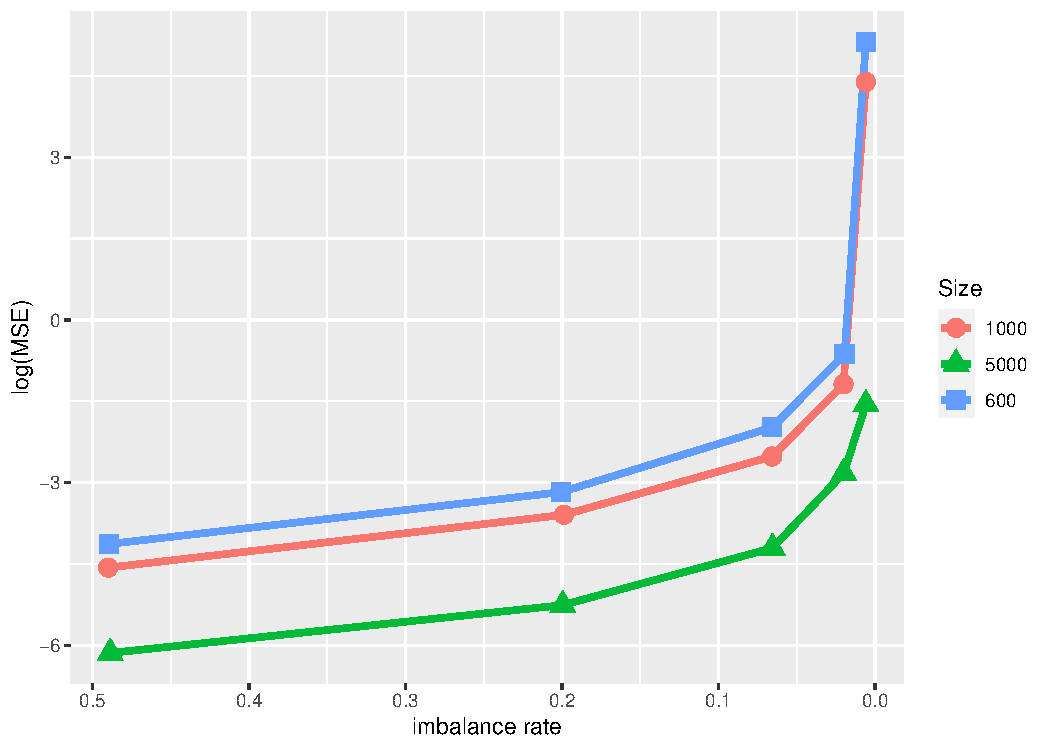
\includegraphics[width=0.8\textwidth]{imbmse.pdf}
        %\caption{MSE}
        \label{fig:imbmse}
    \end{figure}
        
    \end{frame}
%----------------------------------------------------
    \begin{frame}{Effects of imbalance}
    \begin{figure}
	\centering
	\begin{subfigure}{0.47\textwidth}
		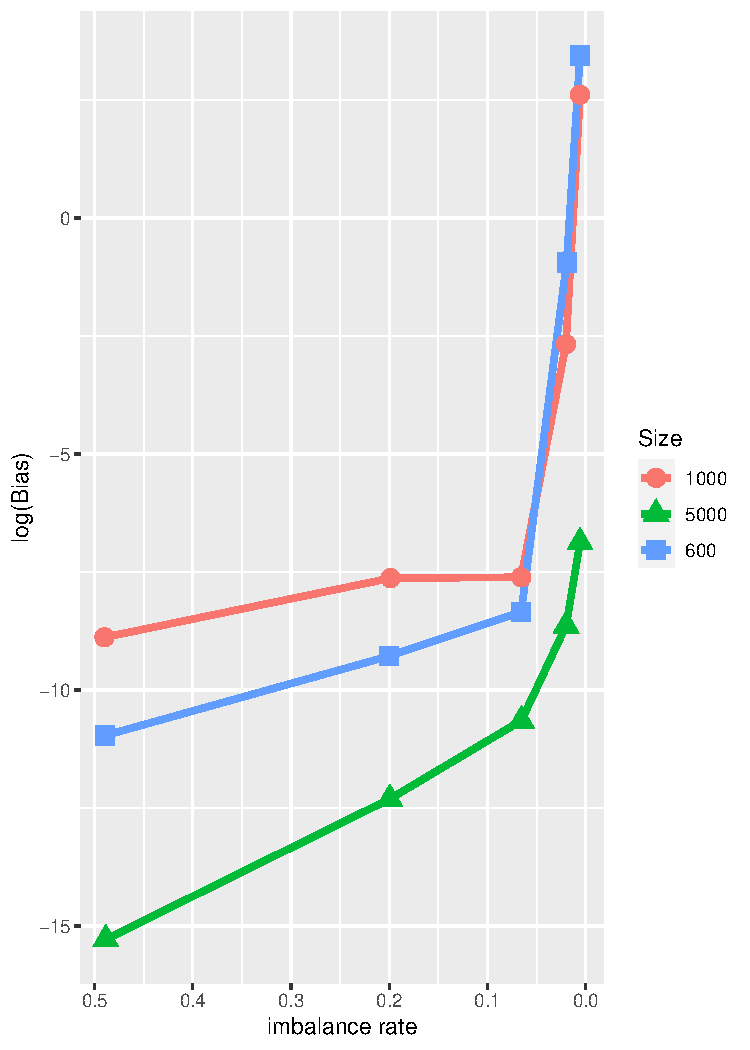
\includegraphics[width=\textwidth]{imbbias.pdf}
		\caption{Bias}
	\end{subfigure}
	\begin{subfigure}{0.47\textwidth}
		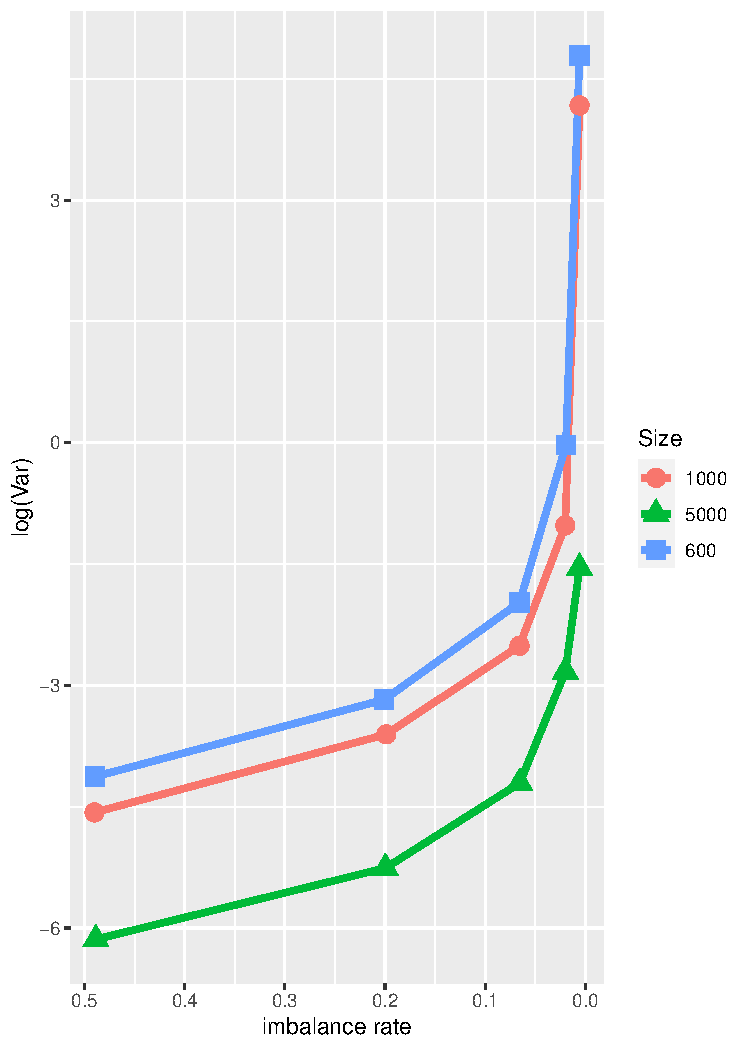
\includegraphics[width=\textwidth]{imbvar.pdf}
		\caption{Variance}
	\end{subfigure}
	%\caption*{Effects of imbalance}
	\label{fig:imb}
	\end{figure}
        
    \end{frame}
    
%--------------------------------------------------
    \begin{frame}{Effects of imbalance}
    \framesubtitle{Relation between MSE and imbalance rate}
    \begin{block}{Convergence rate}
        \begin{equation*}
            \log(N\times\text{MSE})=-\log(\tau)+\log(K)
            \Rightarrow
            \text{MSE}=\frac{K}{\tau N}=\frac{K}{N_1}
        \end{equation*}
    \end{block}
    \begin{figure}
        \centering
        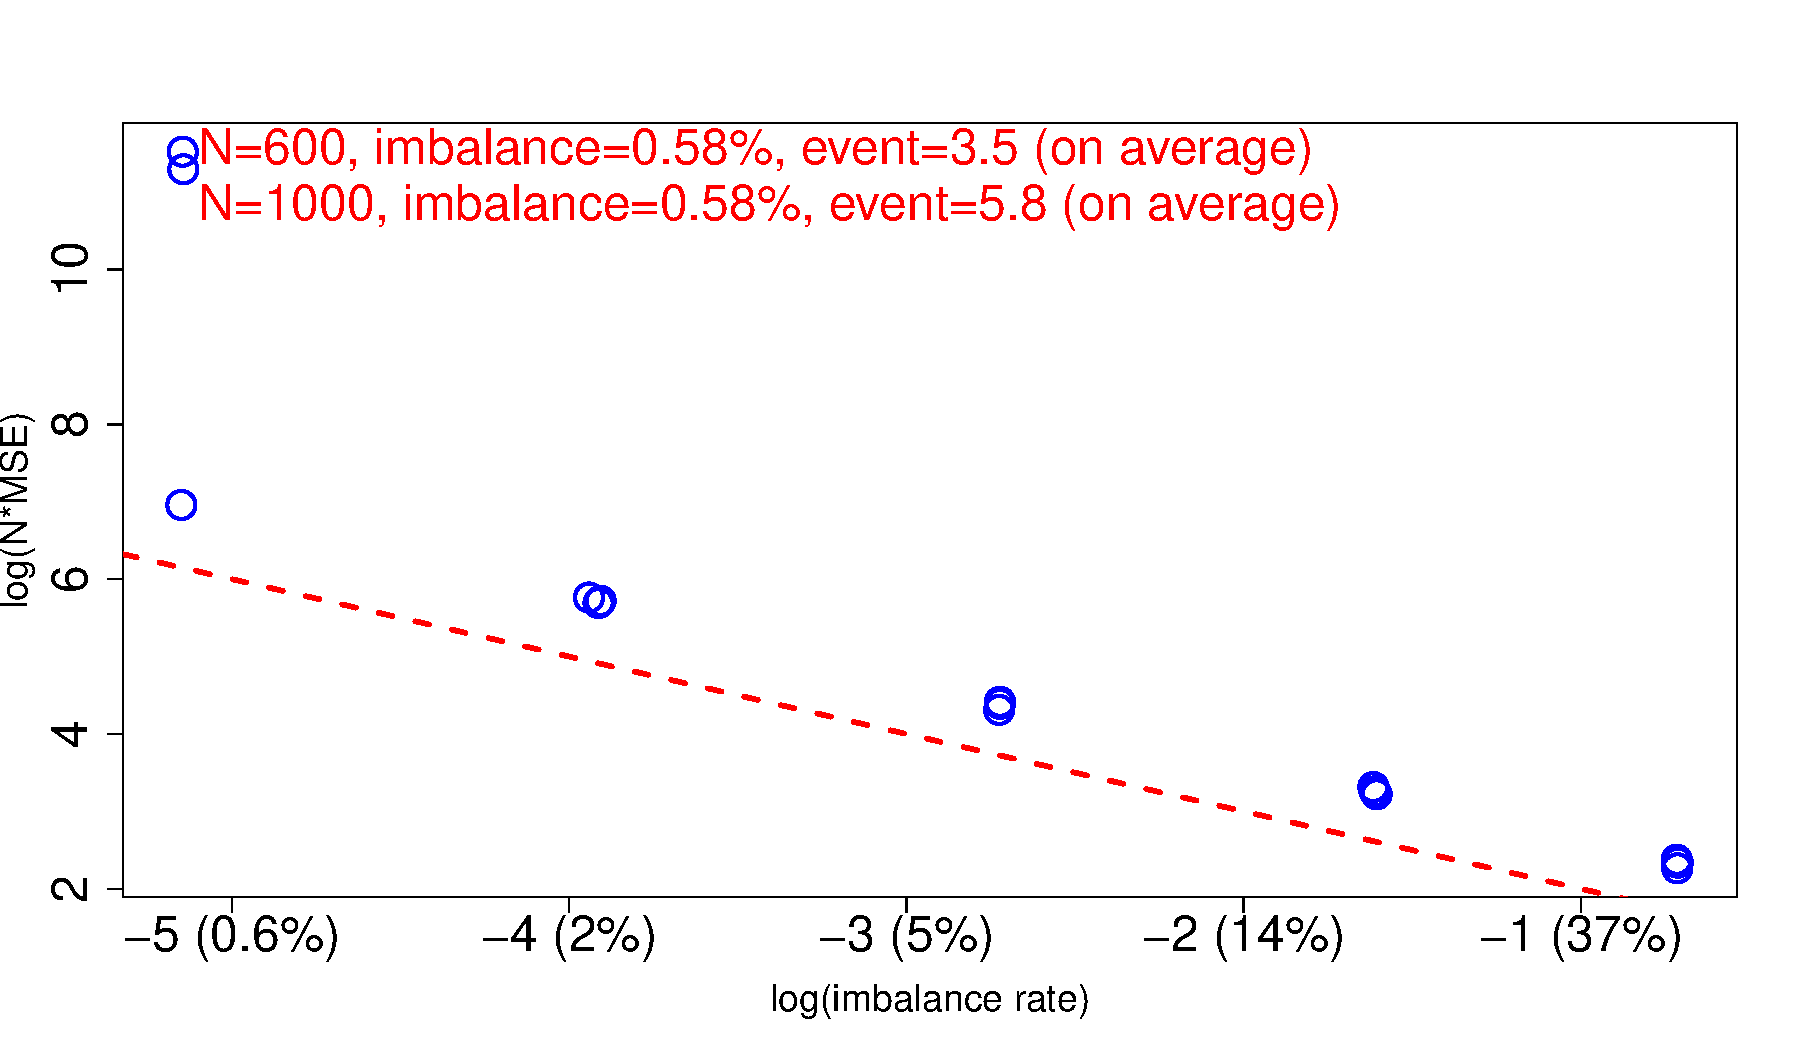
\includegraphics[width=0.9\textwidth]{log-log.pdf}
        %\caption{MSE}
        \label{fig:loglog}
    \end{figure}
    \end{frame}
%---------------------------------------------------
    \subsection{Implication of the results}
    \begin{frame}{Implication of the results}
    \begin{block}{Implication from the simulation}
        \begin{itemize}
            \item High imbalance rate will highly inflate MSE
            \item The amount information is essentially determined by $N_1$
            \item For finite sample, highly imbalance data is hard to analyze since observation of event is not sufficient
        \end{itemize}
    \end{block}
    \end{frame}

    \begin{frame}{Implication of the results}

    \begin{block}{Problem in practice and possible solution}
        \begin{itemize}
            \item Reasonable estimates may involve {\blue massive data} because we need large amount of data to observe sufficient events
            \item For {\blue online system or observed data}, computation complexity maybe heavy for massive data and too waste to record too much censors
            \item Sampling may relief imbalance issue and reduce computational burden
        \end{itemize}
    \end{block}
    \end{frame}
%---------------------------------------------------    
    \section{Balancing data with sampling}
    \begin{frame}{Main idea}
    \framesubtitle{Similarity between logistic regression and Cox model}
        Assuming a proportional hazard model $h(t;\x_i)=h_0(t)e^{\x_i\tp\bbeta}$, for survivial data $\left\{(t_i,\delta_i,\x_i)\right\}_{i=1}^{N}$
        \begin{align*}
            L(\bbeta;\X,\bt,\bdelta)&=\prod_{i=1}^{N}e^{-H(t_i)e^{\x_i\tp\bbeta}}\prod_{i=1}^N\left\{h(t_i)\right\}^{\delta_i}\\
            &=\prod_{i=1}^N \exp\left\{-e^{\log\int_{0}^{t_i}h_0(s)\mathrm{d}s+\x_i\tp\bbeta}\right\}
            \prod_{i=1}^N\left\{e^{\log h_0(t_i)+\x_i\tp\bbeta}\right\}^{\delta_i}.
        \end{align*}
        Assuming that {\blue $h_0(t)$ is very \textbf{small}}, for example, $\log\int_{0}^{t_i}h_0(s)\mathrm{d}s\to-\infty$, we have $e^{\log\int_{0}^{t_i}h_0(s)\mathrm{d}s+\x_i\tp\bbeta}\approx 0$ and thus
        \begin{equation*}
            \exp\left\{-e^{\log\int_{0}^{t_i}h_0(s)\mathrm{d}s+\x_i\tp\bbeta}\right\}
            \approx\frac{1}{1+e^{\log\int_{0}^{t_i}h_0(s)\mathrm{d}s+\x_i\tp\bbeta}},
        \end{equation*}
        since {\blue $e^{-x}\approx \frac{1}{1+x}$}, when $x\to 0$.
    \end{frame}

%---------------------------------------------------    
    \begin{frame}{Main idea}
    \framesubtitle{Similarity between logistic regression and Cox model}
    Now, we have the likelihood function of $\left\{(t_i,\delta_i,\x_i)\right\}_{i=1}^{N}$ is
    \begin{equation*}
        L(\bbeta;\X,\bt,\bdelta)\approx
        \prod_{i=1}^N \frac{1}{1+e^{\log\int_{0}^{t_i}h_0(s)\mathrm{d}s+\x_i\tp\bbeta}}
            \prod_{i=1}^N\left\{e^{\log h_0(t_i)+\x_i\tp\bbeta}\right\}^{\delta_i}.
    \end{equation*}
        The likelihood function of logistic regression of $\left\{(y_i,\x_i)\right\}_{i=1}^{N}$
        \begin{equation*}
            L(\bbeta;\X,\y)=\prod_{i=1}^{N}\frac{1}{1+e^{\alpha_i+\x_i\tp\bbeta}}\prod_{i=1}^N\left(e^{\alpha_i+\x_i\tp\bbeta}\right)^{y_i},
        \end{equation*}
    if $\alpha_i$ are different (commonly used as \textit{offset} option in R).
    \begin{block}{Implication}
    \begin{itemize}
        \item The likelihoods are similar for {\blue imbalanced survival data}
        \item Maybe methodology for {\blue balancing binary data} can be used for {\blue imbalanced survival data}.
    \end{itemize}
    \end{block}
    \end{frame}

%---------------------------------------------------
    \subsection{Methodology}
    \begin{frame}{Methodology}
    \framesubtitle{Sampling techniques}
    \begin{itemize}
        \item Remember that {\red\textbf{events}} are essential information
        \item We propose to use under-sampling method because it reduces computational complexity
        \item {\blue\textbf{Under sampling}} is widely used in {\blue binary data} and proposed in \cite{nir2023analyzing} for {\blue survival data}
    \end{itemize}
    \begin{exampleblock}{Under-sampling for survivial data}
        \begin{itemize}
            \item If $\delta_i=1$, include $(t_i, \delta_i, \x_i)$ into the sample
            \item If $\delta_i=0$, include $(t_i, \delta_i, \x_i)$ with probability $\rho$
        \end{itemize}
    \end{exampleblock}
    \end{frame}


    \begin{frame}{Methodology}
    \framesubtitle{Sampling techniques}
    \begin{block}{Features of under-sampling}
        \begin{itemize}
        \item The resultant sample is of size $N_1+\rho N_0$
        \item We can set $\rho$ by ourselves to balance the data as we need
        \item The resultant estimator is usually {\red biased} due to different sampling probability between $0$ and $1$ 
        \item Easy to apply to massive data and streaming data
    \end{itemize}
    \end{block}    
    \end{frame}

%---------------------------------------------------
\begin{frame}{Methodology}
    \framesubtitle{Estimation techniques}
    To debias {\blue\textbf{Cox regression}}, we can use {\red \textbf{weighted method}}
    \begin{block}{Weighted method}
        \begin{itemize}
            \item For sampled data, we weight censors with $\frac{1}{\rho}$
            \item This is essentially approximating the original likelihood and thus should be similar with full data MLE.
            \item Proposed in \cite{nir2023analyzing}.
        \end{itemize}
    \end{block}
    \hspace*{\fill}\\
    \hspace*{\fill}\\
    \begin{itemize}
        \item If $\rho$ is small (usually for imbalanced data), the variance will be inflated
        \item We give censors more weights, which is not reasonable
    \end{itemize}
    \end{frame}
%---------------------------------------------------
\begin{frame}{Methodology}
    \framesubtitle{Estimation techniques}
    Remember that we mentioned similarity between logistic regression and Cox regression. Let $\nu_i$ denote the indicator that if $i$-th data is sampled. We have
    \begin{align*}
        \pr(y_i=1|\x_i,\nu_i=1)&=\frac{\pr(\nu_i=1|y_i=1,\x_i)\pr(y_i=1|\x_i)}{\sum_{t=0}^1\pr(\nu_i=t|y_i=t,\x_i)\pr(y_i=t|\x_i)}\\
        &=\frac{e^{\alpha-\log\rho+\x_i\tp\bbeta}}{1+e^{\alpha-\log\rho+\x_i\tp\bbeta}}
    \end{align*}
    The likelihood of sampled data is 
    \begin{equation*}
        \prod_{i=1}^{N^{*}}\pr(y_i=1|\x_i,\nu_i=1)=\prod_{i=1}^{N^{*}}\frac{1}{1+e^{\alpha-\log\rho+\x_i\tp\bbeta}}\prod_{i=1}^{N^{*}}\left(e^{\alpha-\log\rho+\x_i\tp\bbeta}\right)^{y_i}
    \end{equation*}
    \begin{itemize}
        \item Only the intercept term is different
    \end{itemize}
\end{frame}
%--------------------------------------------------
\begin{frame}{Methodology}
    \framesubtitle{Estimation techniques}
    \begin{itemize}
        \item For logistic regression, we only need to adjust intercept term
        \item For Cox regression, we only estimate $\bbeta$ and do not care $h_0(t)$
        \item Maybe it is possible to directly apply Cox regression on sampled data
    \end{itemize}
    \begin{exampleblock}{Weighted method}
        \begin{itemize}
            \item Taking samples with negative sampling with user-defined $\rho$
            \item Weighting censors with $\frac{1}{\rho}$, apply weighted Cox regression on sample
        \end{itemize}
    \end{exampleblock}
    \begin{exampleblock}{Unweighted method}
        \begin{itemize}
            \item Taking samples with negative sampling with user-defined $\rho$
            \item Directly apply Cox regression on the sample
        \end{itemize}
    \end{exampleblock}
\end{frame}
%--------------------------------------------------
\subsection{Simulation results}
    \begin{frame}{Estimation efficiency}
    \begin{figure}
	\centering
	\begin{subfigure}{0.47\textwidth}
		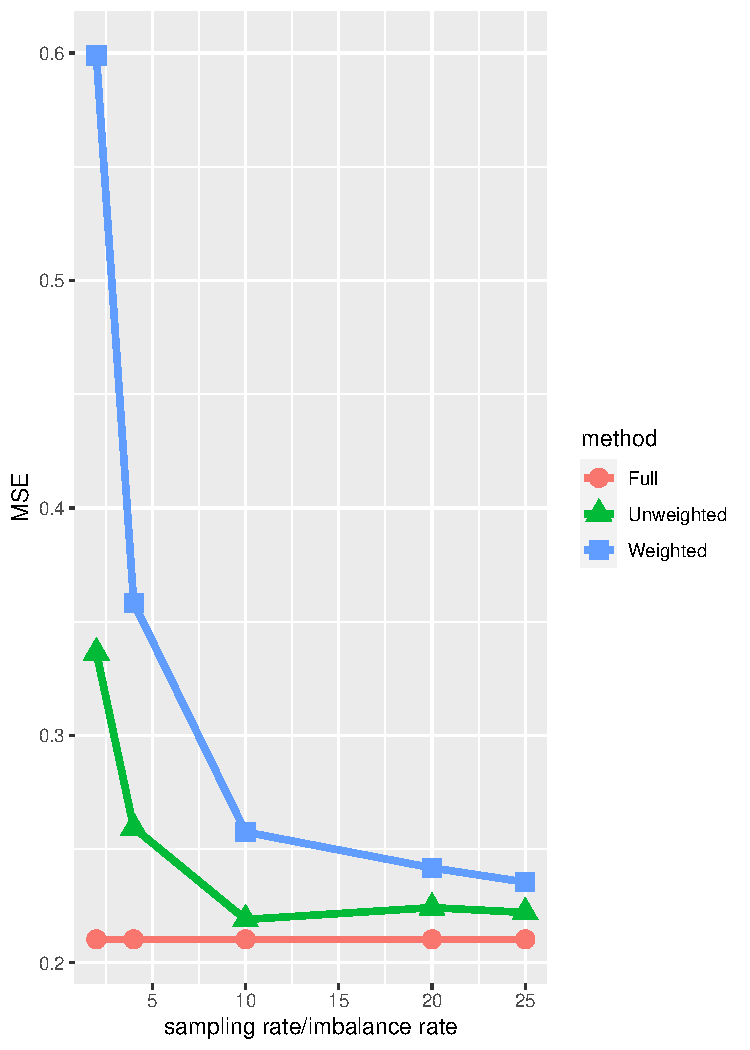
\includegraphics[width=\textwidth]{mse2.pdf}
		\caption{MSE}
	\end{subfigure}
	\begin{subfigure}{0.47\textwidth}
		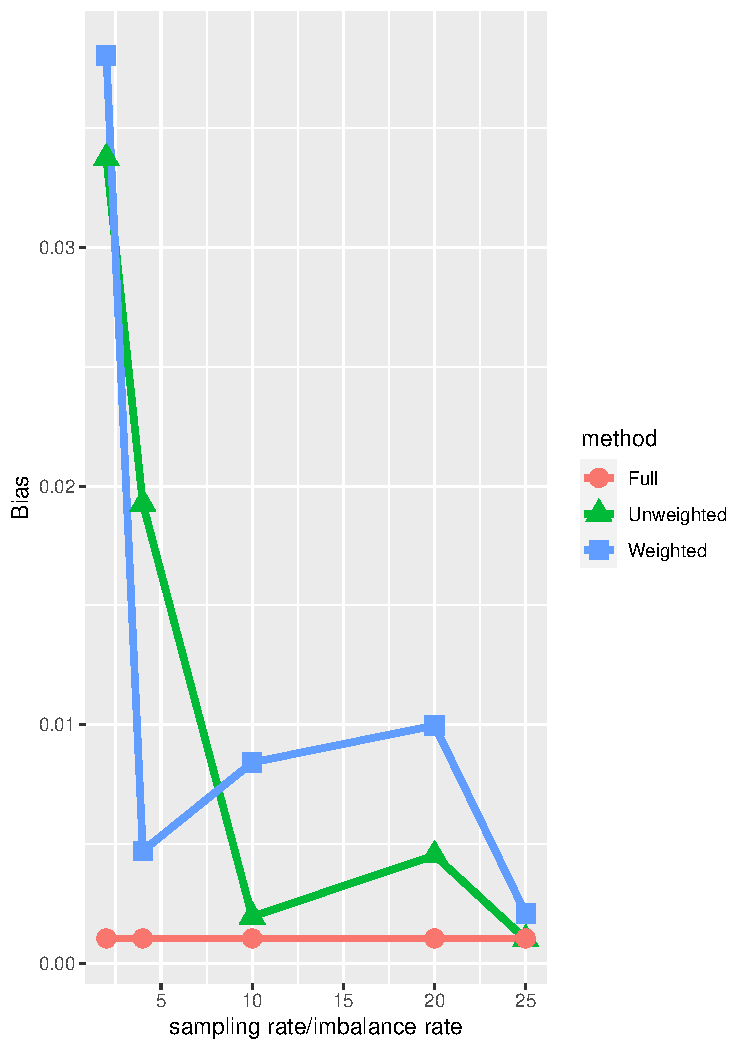
\includegraphics[width=\textwidth]{bias2.pdf}
		\caption{Bias}
	\end{subfigure}
	%\caption*{Effects of imbalance}
	\label{fig:imb}
	\end{figure}
    \end{frame}
%----------------------------------------------------
\begin{frame}{Consistent inferential results}
    % \begin{exampleblock}{Full data}
    % \begin{minted}{R}
    % Call:
    % coxph(formula = Surv(eventtime, status) ~ age + trt + biomk, 
    %     data = dat)

    %           coef exp(coef) se(coef)      z      p
    % age   -0.19684   0.82132  0.08813 -2.233 0.0255
    % trt   -0.71910   0.48719  0.38426 -1.871 0.0613
    % biomk  0.14332   1.15410  0.18204  0.787 0.4311

    % Likelihood ratio test=9.38  on 3 df, p=0.02466
    % n= 5000, number of events= 31
    % \end{minted}
    % \end{exampleblock}
    \begin{figure}
	\centering
	\begin{subfigure}{0.47\textwidth}
		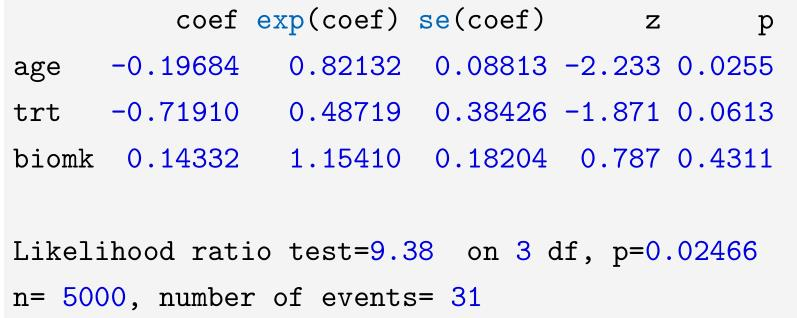
\includegraphics[width=\textwidth]{fit.jpg}
		\caption{Full}
	\end{subfigure}
	\begin{subfigure}{0.47\textwidth}
		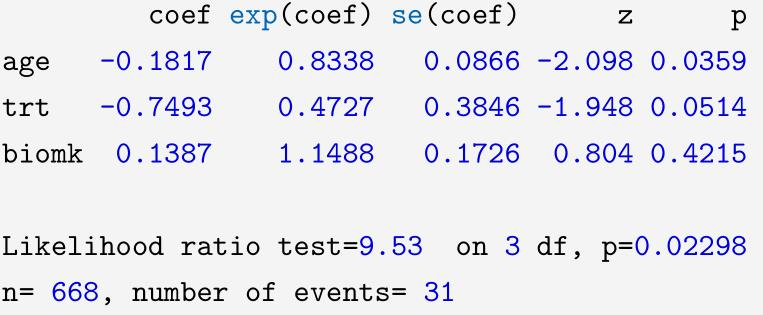
\includegraphics[width=\textwidth]{fituw.jpg}
		\caption{Unweighted}
	\end{subfigure}
    \begin{subfigure}{0.47\textwidth}
		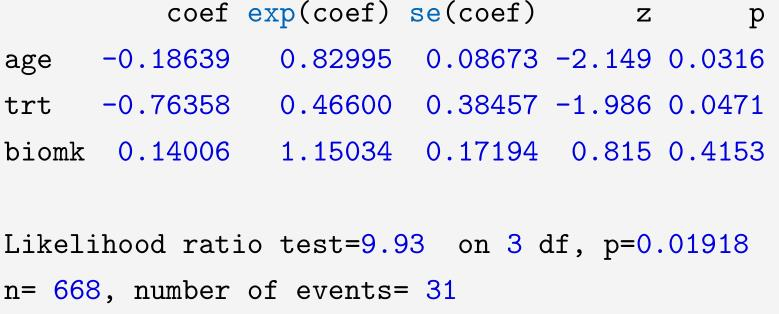
\includegraphics[width=\textwidth]{fitw.jpg}
		\caption{Weighted}
	\end{subfigure}
	%\caption*{Effects of imbalance}
	\label{fig:infer}
	\end{figure}
    \begin{itemize}
        \item When $\frac{N_0}{N_1}=25$ in resultant sample, inference are also very similar 
        \item We only use {\red 668} observations instead of {\red 5000}
    \end{itemize}
\end{frame}
%----------------------------------------------------
\subsection{Computational complexity}
\begin{frame}{Computational complexity}
    \begin{table}[H]
    \caption{Computaional time (in seconds)}
    \label{tab:time}
    \begin{tabular}{cccc}\hline
    \multicolumn{1}{l}{Sampling rate} & Unweighted & Weighted & Full data \\\hline
    0.02                              & 3.92       & 4.37     & 26.65     \\
    0.05                              & 4.47       & 4.73     & 26.65     \\
    0.125                             & 6.38       & 7.00     & 26.65     \\\hline
    \end{tabular}
    \end{table}
    \begin{itemize}
        \item Computational time reduced a lot if use a small sample 
    \end{itemize}
    \hspace*{\fill}\\
    \hspace*{\fill}\\
    \begin{itemize}
        \item This will be more attractive for massive streaming data if we also use an online version of Cox regression because we can reject a lot of censors without losing too much estimation efficiency
    \end{itemize}
    \end{frame}
        %------------------------------------------------

	%\begin{frame}
            %\frametitle{Results and Discussions}
		%\framesubtitle{Select tuning parameter}
        %\begin{itemize}
           %\item Sampling: pixel value
        %\end{itemize}
        %\begin{itemize}
          % \item MM: rank limit 100
      %  \end{itemize}
  		%\begin{figure}
		%	\centering
		%	\begin{subfigure}{0.46\textwidth}
		%		\includegraphics[width=\textwidth,page=1]{lambda/lambda.pdf}
		%	\end{subfigure}
		%	\begin{subfigure}{0.46\textwidth}
		%		\includegraphics[width=\textwidth,page=2]{lambda/lambda.pdf}
				%\caption{Responses are imbalanced}
		%	\end{subfigure}
			%\caption{eMSE for different subsampe sizes $r$ with a pilot sample size $r_{\mathrm{p}}=500$ for logistic regression under different settings.}
		%	\label{fig:lambda}
	%	\end{figure}
		
	%\end{frame}
%------------------------------------------------
        \section{Conclusions}
%------------------------------------------------
	\begin{frame}
		\frametitle{Conclusions}
        Conclusion for this project:
		\begin{itemize} 
            \item Imbalance may cause estimation issue for Cox regression
            \item Balancing methods for classification can be applied to survival data
            \item It is even possible to obtain similar results with very small data size when dealing with massive imbalance survival data
	    \end{itemize}
        Future extension for this project:
        \begin{itemize}
            \item We limited our scope to large scale imbalance data. For finite sample size, it may need other techniques for example, penalization methods
            \item Nonuniform sampling can be considered
            \item Combining negative sampling with online updating of Cox regression maybe interesting and of practical interests.
        \end{itemize}

       \end{frame}
%------------------------------------------------	
	\begin{frame}[noframenumbering, allowframebreaks]
		\frametitle{References}
		\bibliographystyle{natbib}
        \bibliography{reference}
	\end{frame}	
%------------------------------------------------
	
	\begin{frame}
		\Huge{\centerline{Thank you!}}
	\end{frame}
	
	%----------------------------------------------------------------------------------------
	
\end{document}
%%% Local Variables:
%%% TeX-master: t
%%% fill-column: 80
%%% eval: (auto-fill-mode 1)
%%% TeX-command-extra-options: "-shell-escape"
%%% End:
